\documentclass{report}

\usepackage{ugentstyle}



\begin{document}
	\maketitle{Besturingssystemen III}

	\tableofcontents

	\part{Theorie}
	\chapter{WMI concepten}
	\section{Herhaling SNMP en inleiding WMI}
	SNMP had de mogelijkheid om informatie bij te houden van devices die typisch op een netwerk aangesloten zijn zoals printers, routers, workstations en servers. Er was echter nood aan een systeem dat ook informatie van het hele operating systeem kon bevragen.
	Dit systeem noemt \textit{Wbem}, een uniform systeem voor het bevragen van besturingssystemen zoals windows, HP en solaris. Een Windows specifieke versie hiervan is het \textit{Windows Management Instrumentation} (WMI).
	\begin{figure}[h]
		\centering
		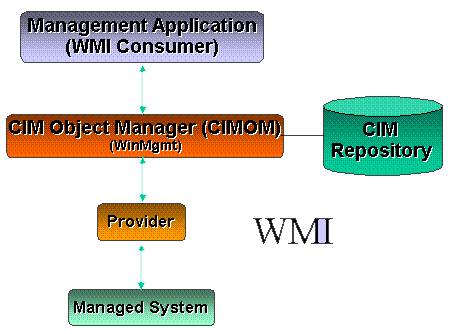
\includegraphics[width=0.5\textwidth]{basisarchitectuur_WMI}
		\caption{Basisarchitectuur WMI}
		\label{fig:basisarchitectuur_WMI}
	\end{figure}

	Uit figuur \ref{fig:basisarchitectuur_WMI} kunnen vijf componenten afgeleid worden:
	\begin{itemize}
		\item \textit{WMI Consumer}
		\item \textit{CIM Object Manager}
		\item \textit{CIM Repository}. Dit is een object geörienteerd model waarbij software als hardware componenten als objecten voorgesteld worden. 
		\item \textit{Provider}
		\item \textit{Managed System}
	\end{itemize}
	\section{CIM Repository}
	De CIM Repository kan men inspecteren met een WMI-browser. Voorbeelden hiervan zijn \textit{WMI CIM Studio} en \textit{Powershell WMI Browser}. In deze samenvatting wordt gebruik gemaakt van WMI CIM Studio
	De inlogprocedure vraagt een namespace die standaard ingevuld staat op \texttt{root:\\CIMV2}. Deze namespace omvat ook de meeste WMI Objecten. Wat deze namespace niet heeft zijn klassen om office documenten zoals excel of word te manipuleren.
	Indien ingelogd, verschijnt er een scherm met twee panelen. Het linkerpaneel bevat alle klassen gesorteerd op hiërarchische volgorde op basis van overerving. De icoontjes naast elke klasse wordt gegenereerd op basis attributen van die klasse.
	Het rechterpaneel heeft standaard de \textit{Properties} tab open. Dit tabblad bevat alle attributen van de geselecteerde klasse. Attributen voorafgegaan door 2 underscores zijn systeemattributen en bestaan voor elke klasse.
	Voorbeelden van zulke systeemattributen:
	\begin{itemize}
		\item \_\_DERIVATION : Dit bevat een tabel met de hiërarchie van de overerving waarbij het eerste element de onmiddelijke superklasse is en het laatste element de root van de hiërarchie.
		\item \_\_DYNASTY : Dit bevat de root van de hiërarchie van overerving. Deze informatie is dus dezelfde als het laatste element in het \_\_DERIVATION attribuut.
		\item \_\_PROPERTY\_COUNT : Dit veld bevat een nummer met het aantal niet-systeemaanroepen
		\item \_\_PATH : Dit veld bevat het absolute pad van de klasse.
	\end{itemize}
	Van elke klasse kan zijn instanties opgevraagd worden door op het icoontje rechts van het save-icoontje te klikken. Er wordt een twee dimensionale tabel weergegeven met per instantie een rij en per attribuut een kolom.
	Voor elke instantie moet het systeemattribuut \_\_RELPATH aangevuld worden met de sleutel van het object. Dit is een string dat bestaat uit meerdere key-value paren dat toegevoegd wordt aan de default waarde van \_\_RELPATH.
	Bij Singletons echter zijn unieke identificaties niet nodig en wordt \_\_RELPATH aangevuld met een \@ symbool. Een voorbeeld van een abstracte klasse en een singleton is respectievelijk \texttt{CIM\_MonitorResolution} en \texttt{Win\_LocalTime}. 
	\subsection{Qualifiers}
	Een qualifier is een key-value koppel waarbij extra eigenschappen kunnen toegevoegd worden. Er bestaan vier soorten qualifiers:
	\begin{enumerate}
		\item klasse-qualifiers. Geeft extra informatie over de klasse. 
		\item attribuut-qualifiers. Geeft extra informatie over de attributen van een klasse
		\item methode-qualifiers. Geeft extra informatie over de methoden van een klasse
		\item methodeparameter-qualifiers. Geeft extra informatie over de parameters van de methoden van een klasse.
	\end{enumerate}
	\subsubsection{Klasse-qualifiers}
	Deze worden in WMI CIM Studio \textit{Object qualifiers} genoemd:
	\begin{itemize}
		\item De \textit{Description} qualifier geeft tekst terug met informatie over de klasse.
		\item De \textit{Abstract}, \textit{Dynamic} en \textit{Singleton} qualifiers geven aan, indien hun waarde op \textit{true} staat, dat een klasse abstract, dynamisch of een singleton is.
		\item De \textit{Provider} qualifier helpt de WMI service te bepalen welke provider moet aangesproken worden om een bepaalde klasse aan te spreken
	\end{itemize}
	\subsubsection{Attribuut-qualifiers}
	De attribuut-qualifiers worden in WMI CIM Studio \textit{Property qualifiers} genoemd:
	\begin{itemize}
		\item De \textit{Description} qualifier geef analoog zoals de klasse-qualifiers tekst terug met informatie over het attribuut.
		\item De \textit{CIMType} qualifier geeft het type van het attribuut weer, zoals string, boolean, datetime, signed of unsigned int (8, 16, 32 of 64 bits) of referenties naar absolute objectpaden.
		\item De \textit{Write} qualifier geeft aan, indien deze op \textit{true} staat, dat de het attribuut rechtstreeks wijzigbaar is, zonder hiervoor methodes te moeten aanspreken. 
		\item De \textit{Keys} qualifier geeft aan dat het attribuut deel uitmaakt van de sleutel van het object en bijgevolg ook vermeld moet worden in het objectpad van een instantie.
		\item ValueMap geeft in een ééndimensionale tabel het domein weer van het attribuut: een expliciete opsomming van de toegelaten waarden.
			  Values geeft een meer informatieve interpretatie van de toegelaten waarden. Indien ook de ValueMap qualifier aanwezig is, kunnen ValueMap en Values best beschouwd worden als respectievelijk de keys en de values van een Perl hash. Indien een ValueMap ontbreekt, dan impliceert Values een ValueMap met oplopende gehele getallen, startend vanaf 0. Values kan dan geïnterpreteerd worden als een Perl array.
	\end{itemize}
	\part{Examenvragen}
	\chapter{Modelvragen theorie: reeks A}
	Het examen wordt \accentuate{volledig schriftelijk} beantwoord. Indien de student dit wenst, wordt het antwoord onmiddellijk na indienen geëvalueerd, en eventueel gevolgd door enkele vragen ter verduidelijking of aanvulling.
	
	\section{Structuur van Active Directory gegevens}
	\begin{enumerate}
		\item Bespreek de \textit{diverse namen} die alle Active Directory objecten \textit{identificeren}. \accentuate{\textsection 2.2.1}
		
		\item Wat zijn \textit{SPN objecten} ? Bespreek de \textit{aanvullende naamgeving} voor deze objecten. \accentuate{ (\textsection 2.2.2)}
		
		\item Enkele veel gebruikte klassen (hiermee worden \textit{attributeschema} en \textit{classschema} objecten niet bedoeld) vertonen nog meer identificerende attributen voor hun instanties. Bespreek deze klassen en attributen.
		
		\item In welke \textit{partities} is de Active Directory informatie verdeeld ? Geef de betekenis van elke partitie, hun onderlinge relatie (zowel fysiek als met betrekking tot hun naamgeving), en de replicatiekarakteristieken ervan. \accentuate{(laatste helft \textsection 2.2.3)}
	\end{enumerate}

	\section{attributeSchema objecten \accentuate{ (\textsection 2.2.4 en \textsection 2.2.5)}}
	\begin{enumerate}
		\item Bespreek het \textit{doel} en de \textit{werking} van attributeSchema objecten. Hoe kunnen deze objecten het best \textit{geraadpleegd} en \textit{gewijzigd} worden ?
		
		\item Bespreek de \textit{diverse naamgevingen}, specifiek voor attributeSchema objecten.
		
		\item Bespreek de belangrijkste \textit{kenmerken} van attributeSchema objecten, en op welke waarden die ingesteld kunnen worden.
		
		\item Welke andere types objecten bevat het \textit{Active Directory schema}, en wat is hun bedoeling ? \accentuate{ (o.a. \textsection 2.2.7)}
		
		\item Via welke attributen kun je de \textit{klasse} van een willekeurig Active Directory object achterhalen ? Hoe moet je op zoek gaan naar alle objecten van een bepaalde klasse ? Illustreer aan de hand van relevante voorbeelden. \accentuate{ (laatste paragraaf \textsection 2.2.6)}
	\end{enumerate}

	\section{classSchema objecten \accentuate{ (\textsection 2.2.4 en \textsection 2.2.6)}}
	\begin{enumerate}
		\item Bespreek het \textit{doel} en de \textit{werking} van classSchema objecten.
		
		\item Hoe benadert Active Directory het mechaniscme van \textit{overerving} ?
		
		\item Bespreek de diverse \textit{naamgevingen}, specifiek voor classSchema objecten.
		
		\item Bespreek de belangrijkste \textit{kenmerken} van classSchema objecten, en op welke waarden die ingesteld kunnen worden.
		
		\item Welke andere types objecten bevat het \textit{Active Directory schema}, en wat is hun bedoeling ? \accentuate{ (o.a. \textsection 2.2.7)}
		
		\item Hoe en met welke middelen kan het Active Directory schema uitgebreid worden ? Waarom moet je en hoe kan je hierbij \textit{voorzichtig} te werk gaan ? \accentuate{ (o.a. \textsection 2.2.8, ldifde fractie \textsection 2.2.3)}
	\end{enumerate}

 	\section{Active Directory domeinstructuren \accentuate{(§2.4.4, laatste paragraaf §2.4.5 en §2.4.6)}}
 	\begin{enumerate}
 		\item Wat is de bedoeling van \textit{vertrouwensrelaties} ?
 		
 		\item Bespreek de verschillende \textit{soorten} vertrouwensrelaties.
 		
 		\item Op welke diverse manieren kunnen vertrouwensrelaties \textit{gecreëerd} en \textit{gecontroleerd} worden ? Bespreek ook de \textit{optionele configuratiemogelijkheden}.
 		
 		\item Welke verschillen zijn er in praktijk tussen \textit{NT 4.0} en \textit{Windows Server} domeinstructuren ? Bespreek onder andere telkens de noodzaak om meerdere domeinen in te voeren. Bespreek de alternatieve mogelijkheden bij de \textit{conversie van een NT 4.0 domeinstructuur} naar een Windows Server omgeving.
 	\end{enumerate}
 
 	\section{Active Directory server rollen \accentuate{(§2.4.7, §2.3 en fractie §2.4.2)}}
 		Welke vragen moet men zich stellen na de initiële installatie van een Windows Server toestel, in verband met \textit{bijzondere functies} die de server kan vervullen met betrekking tot Active Directory ? Formuleer bij het beantwoorden van deze vragen telkens (voor zover relevant): 
 		\begin{enumerate}
 			\item Hoe bepaald wordt \textit{welke servers} een dergelijke specifieke functie vervullen ? \textit{Hoeveel} zijn er nodig (in termen van: \textit{minimaal/exact/maximaal} \#, \textit{in functie van} ...), en waarom ?
 		
 			\item \textit{Eigenschappen} zoals bedoeling, noodzaak, kriticiteit, inhoud, synchronisatie, voor welke Windows versie(s) van toepassing, ... ?
 		
 			\item De \textit{eventuele relatie} tussen de diverse functies. Vermeld bijvoorbeeld welke functies al dan niet door dezelfde server \textit{kunnen} vervuld worden, of misschien wel juist wel door dezelfde server \textit{moeten} vervuld worden.
 		
 			\item Hoe kan achterhaald worden welk(e) toestel(len) de bijzondere functie vervult, en op welke diverse manieren men de \textit{toewijzing} ervan kan instellen, wijzigen en/of ongedaan maken ?
 		\end{enumerate}	
	\chapter{Modelvragen theorie: reeks B}
	\section{Active Directory functionele niveaus \accentuate{(§2.4.3)}}
	\begin{enumerate}
		\item Geef de diverse \textit{functionele niveaus} waarop Active Directory kan ingesteld worden, en welke beperkingen er het gevolg van zijn.
		\item Bespreek van elk niveau alle eraan gekoppelde voordelen. Geef hierbij telkens een korte bespreking \accentuate{(verspreid over de cursus !)} van ingevoerde begrippen.
		
		\item Hoe kan men detecteren op welk niveau een Active Directory omgeving zicht bevindt ?
		
		\item Op welke diverse manieren kan men het functionele niveau verhogen of verlagen ?
	\end{enumerate}
	
	\section{Active Directory replicatie \accentuate{(§2.5)}}
	\begin{enumerate}
		\item Wat is de bedoeling van \textit{replicatie} ?
		
		\item Hoe wordt dit in Windows Server (ondermeer ten opzichte van NT 4.0) gerealiseerd: bespreek de verschillende \textit{technische kenmerken} en \textit{concepten} van Windows Server replicatie, en hoe men specifieke problemen vermijdt of oplost.
		
		\item Welke toestellen repliceren onderling in een \textit{forest} ? Welke specifieke gegevens worden hierbij uitgewisseld ?
		
		\item Welke impact hebben \textit{sites} met betrekking tot de replicatie van Active Directory gegevens ? Welke andere Active Directory aspecten worden door sites beïnvloed ? \accentuate{(§2.6.1)}
		
		\item Hoe wordt bepaald \textit{tot welke site} computers, servers in het bijzonder, behoren ? \accentuate{(laatste paragraaf §2.6.2 en fractie §2.6.3)}
	\end{enumerate}

	\section{Gedeelde mappen en NTFS}
	\begin{enumerate}
		\item Welke \textit{configuratieinstellingen} kun je maken tijdens of onmiddellijk na het creëren van gedeelde mappen ? Bespreek het \textit{doel} van elk van deze diverse instellingen en de belangrijkste \textit{eigenschappen} en \textit{mogelijkheden} ervan. \accentuate{(§3.2.1, §3.2.2, fracties §3.3.1, §3.4.2, §3.4.3, §3.5 en §3.6)}
		
		\item Waar wordt de definitie en (partiële) configuratie van gedeelde mappen \textit{opgeslagen} ? Hoe kan men deze wijzigen vanuit een \textit{Command Prompt} ? 
		
		\item Geef een overzicht van de belangrijkste voordelen van de opeenvolgende versies van het \textit{NTFS bestandssysteem}. Bespreek elk van deze aspecten (ondermeer het doel, de voordelen en de beperkingen ervan), en geef aan hoe je er gebruik kan van maken, bij voorkeur vanuit een \textit{Command Prompt}. \accentuate{(NTFS fractie §1.6, fracties §3.4.1, §3.4.2 en §3.4.4)}
	\end{enumerate}

	\section{Machtigingen op bestandstoegang \accentuate{(§3.3)}}
	\begin{enumerate}
		\item Welke rol spelen machtigingen bij de beveiliging van bronnen ? Geef een gedetailleerd overzicht van het \textit{algemeen} (op alle windows objecten toegepast) mechanisme van \textit{machtigingen}.
		
		\item Bespreek hoe het mechanisme van machtigingen \textit{specifiek} (en op diverse niveaus) \textit{toegepast} wordt op \textit{bestandstoegang}. Geef de verschillende soorten machtigingen, hun onderlinge relaties, en hoe deze kunnen \textit{geanalyseerd} en \textit{ingesteld} worden. Toon hierbij aan dat je zelf met deze configuratietools geëxperimenteerd hebt.
		
		\item Wat gebeurt er met de machtigingen bij het \textit{verplaatsen} van een bestand ? Wat gebeurt er met de machtigingen bij het \textit{kopiëren} van een bestand ?
		
		\item Op welke \textit{andere objecten} zijn machtigingen van toepassing ?
		
		\item Wie is \textit{in principe} verantwoordelijk voor het configureren van machtigingen ? Door welke instelling is dit zo vastgelegd ? Hoe kan ervoor gezorgd worden dat enkel \textit{administrators} verantwoordelijk gesteld worden voor het configureren van machtigingen ?
		
	\end{enumerate}

	\section{Gebruikersgroepen \accentuate{(§4.2.2 en §4.2.3)}}
	\begin{enumerate}
		\item Bespreek in detail het onderscheid tussen de diverse soorten \textit{veiligheidsgroepen}, ondermeer afhankelijk of het toestel al dan niet in een domein is opgenomen. Behandel hierbij vooral de mogelijkheden en beperkingen. Bespreek ondermeer:
			\begin{itemize}
				\item de \textit{zichtbaarheid} van de diverse soorten groepen,
				\item welke objecten er \textit{lid} van kunnen zijn,
				\item de onderlinge relaties en de regels voor het \textit{nesten} van de diverse soorten groepen ? Stel deze relaties eveneens schematisch voor.
			\end{itemize}
		\item Hoe en waarom worden deze soorten groepen \textit{in de praktijk} best gebruikt, al dan niet gecombineerd ? Van welke omstandigheden is dit afhankelijk ? Illustreer aan de hand van concrete voorbeelden. 
		
		\item Waar en hoe wordt het (volledige) lidmaatschap van een \textit{user} object tot een groep bijgehouden ? Op welke diverse manieren kan men dit lidmaatschap \textit{configureren} ? Op welke diverse manieren kan men de volledige verzameling van objecten, die deel uitmaken van een specifieke groep, of de volledige verzameling van groepen, waar een specifiek object deel van uitmaakt, achterhalen ? \accentuate{ (partim §4.1.2 en §4.2.3)}
		
		\item Door \textit{wie} wordt het lidmaatschap van de diverse groeptypes bij voorkeur ingesteld ?
		
		\item Op welke diverse manieren kan men het beheer van Active Directory objecten, specifieke attributen van groepsobjecten in het bijzonder, \textit{delegeren aan niet-Administrators} ? Bespreek een aantal technieken om dit delegeren \textit{zo eenvoudig mogelijk} uit te voeren. \accentuate{(partim §4.1.2, en §4.4.2)} 
	\end{enumerate}
\end{document}


